\begin{activity} \label{A:4.3.3}  Suppose that $v(t) = \sqrt{4-(t-2)^2}$ tells us the instantaneous velocity of a moving object on the interval $0 \le t \le 4$, where $t$ is measured in minutes and $v$ is measured in meters per minute.
\ba
\item Sketch an accurate graph of $y = v(t)$.  What kind of curve is $y = \sqrt{4-(t-2)^2}$?
\item Evaluate $\int_0^4 v(t) \, dt$ exactly.
\item In terms of the physical problem of the moving object with velocity $v(t)$, what is the meaning of $\int_0^4 v(t) \, dt$?  Include units on your answer.
\item Determine the exact average value of $v(t)$ on $[0,4]$.  Include units on your answer.
\item Sketch a rectangle whose base is the line segment from $t=0$ to $t = 4$ on the $t$-axis such that the rectangle's area is equal to the value of $\int_0^4 v(t) \, dt$.  What is the rectangle's exact height?
\item How can you use the average value you found in (d) to compute the total distance traveled by the moving object over $[0,4]$?
\ea
\end{activity}
\begin{smallhint}
\ba
	\item Note that $y = \sqrt{4-(t-2)^2}$ is part of the curve given by $(t-2)^2 + y^2 = 4$.
	\item What familiar shape is generated by the curve $y = v(t)$?
	\item Recall the meaning of the area bounded by a nonnegative velocity function on a given interval.
	\item From the meaning of the average value of a function, we know $v_{\mbox{\tiny{AVG}}}[a,b] = \frac{1}{b-a}  \int_a^b v(t) \, dt$.
	\item Consider a key recent figure in the text.
	\item Distance equals average rate times $\ldots$.
\ea
\end{smallhint}
\begin{bighint}
\ba
	\item Note that $y = \sqrt{4-(t-2)^2}$ is the top half of the curve given by $(t-2)^2 + y^2 = 4$, which is a familiar one.
	\item What familiar shape is generated by the curve $y = v(t)$?  What known formula for area helps?
	\item Recall the meaning of the area bounded by a nonnegative velocity function on a given interval.  See, for instance, Section~\ref{S:4.1.VelocityDistance}.
	\item From the meaning of the average value of a function, we know $v_{\mbox{\tiny{AVG}}}[a,b] = \frac{1}{b-a}  \int_a^b v(t) \, dt$.  What are $a$ and $b$ in this problem?
	\item Consider a key recent figure in the text and construct a similar drawing for the given function $v$.
	\item Distance equals average rate times time!
\ea
\end{bighint}
\begin{activitySolution}
\ba
	\item The curve $y = v(t) = \sqrt{4-(t-2)^2}$ is the top half of the circle $(t-2)^2 + y^2 = 4$, which has radius 2 and is centered at $(2,0)$.
	\item Thus, the value of $\int_0^4 v(t) \, dt$ is the area of a semicircle of radius 2, which is $\frac{1}{2} \pi (2)^2 = 2\pi$.
	\item Because the velocity $v(t)$ is always nonnegative in this problem, the meaning of $\int_0^4 v(t) \, dt = 2\pi$ is both the distance traveled and the change in position of the object on the interval $0 \le t \le \pi$.  Specifically, the object moved $2 \pi$ meters in 4 minutes.
	\item We know $v_{\mbox{\tiny{AVG}}}[a,b] = \frac{1}{b-a}  \int_a^b v(t) \, dt$, so
	$$v_{\mbox{\tiny{AVG}}}[0,4] = \frac{1}{4-0}  \int_0^4 \sqrt{4-(t-2)^2} \, dt = \frac{1}{4} 2\pi = \frac{\pi}{2},$$
	which is measured in meters per minute, since the units on ``4'' are minutes and on ``$2\pi$'' are meters.
	\item Constructing a figure similar to those shown in this section on the topic of average value of a function, we find the following, which demonstrates a rectangle having the same area as the semicircle.
	\begin{center}
	  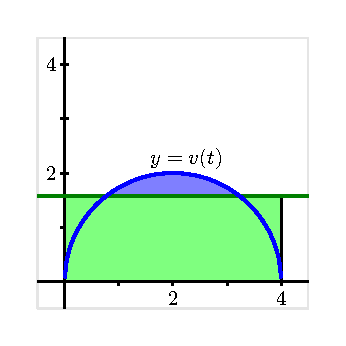
\includegraphics{figures/4_3_Act3Soln.eps}
	\end{center}
	The height of the rectangle is the average value of $v$, specifically $v_{\mbox{\tiny{AVG}}}[0,4] = \frac{\pi}{2} \approx 1.57$.
	\item Knowing that average velocity is $\frac{\pi}{2}$, it follows from the fact that distance traveled equals average rate times time (provided velocity is always nonnegative), we have
	$$D = \frac{\pi}{2} \cdot 4 = 2\pi.$$
	We see from (c) or (f) that we are simply considering the situation from two different perspectives: if we know the distance traveled, we can find average velocity, or if we know average velocity, we can find distance traveled.
\ea
\end{activitySolution}
\aftera





